\chapter{Curve fitting for NNQS}\label{appendix:curvefitting}
This section will describe how we obtained an approximate analytical form of functions $A(s)$ and $B(s)$ as shown in \autoref{dwaveannealing}. The exact form is not provided in the D-wave documentation but a set of 1000 points is available from the documentation \cite{dwavefunctions}. A snapshot of the dataset is shown here:
\begin{table}[!h]
    \centering
    \begin{tabular}{cccc}
    \hline
    $s$ & $A(s)$ (GHz) & $B(s)$ (GHz)\\
    \hline
    0 & 0.000000 & $9.839417 \times 10^0$ \\
    0.001 & 0.001001 & $9.746483 \times 10^0$ \\
    0.002 & 0.002002 & $9.655434 \times 10^0$ \\
    ... & ... & ... \\
    0.998 & 0.997998 & $1.344913 \times 10^{-9}$\\
    0.999 & 0.998999 & $1.293784 \times 10^{-9}$\\
    1.000 & 1.000000 & $1.242656 \times 10^{-9}$\\
    \hline
    \end{tabular}
    \caption{Discrete points of annealing functions $A(s)$ and $B(s)$.}
    \label{tab:dwavefunction}
\end{table}

To obtain an analytical form, we utilised the curve fit function from the scipy library. First, we normalize by the maximum value in $B(s)$ as only the ratio of $A$ and $B$ is We fit an exponential decay form of $a_{A}\cdot e^{-b_{A}\cdot s} + c_{A}$ to $A(s)$ and a quadratic function $a_{B} \cdot s^2 + b_{B} \cdot s + c_{B}$ function to $B(s)$. The forms of the functions were chosen from the D-wave documentation \cite{dwavefunctions}. We obtain fitted constants of $a_{A}=1.11, b_{A} = 7.06, c_A-0.00569, a_B = 0.680, b_B = 0.288, c_B = 0.0305$. The fitted functions are shown in \autoref{fittedequation} along with the discrete values from the documentation and are found to be a good fit.
\begin{figure}[!h]
    \centering
    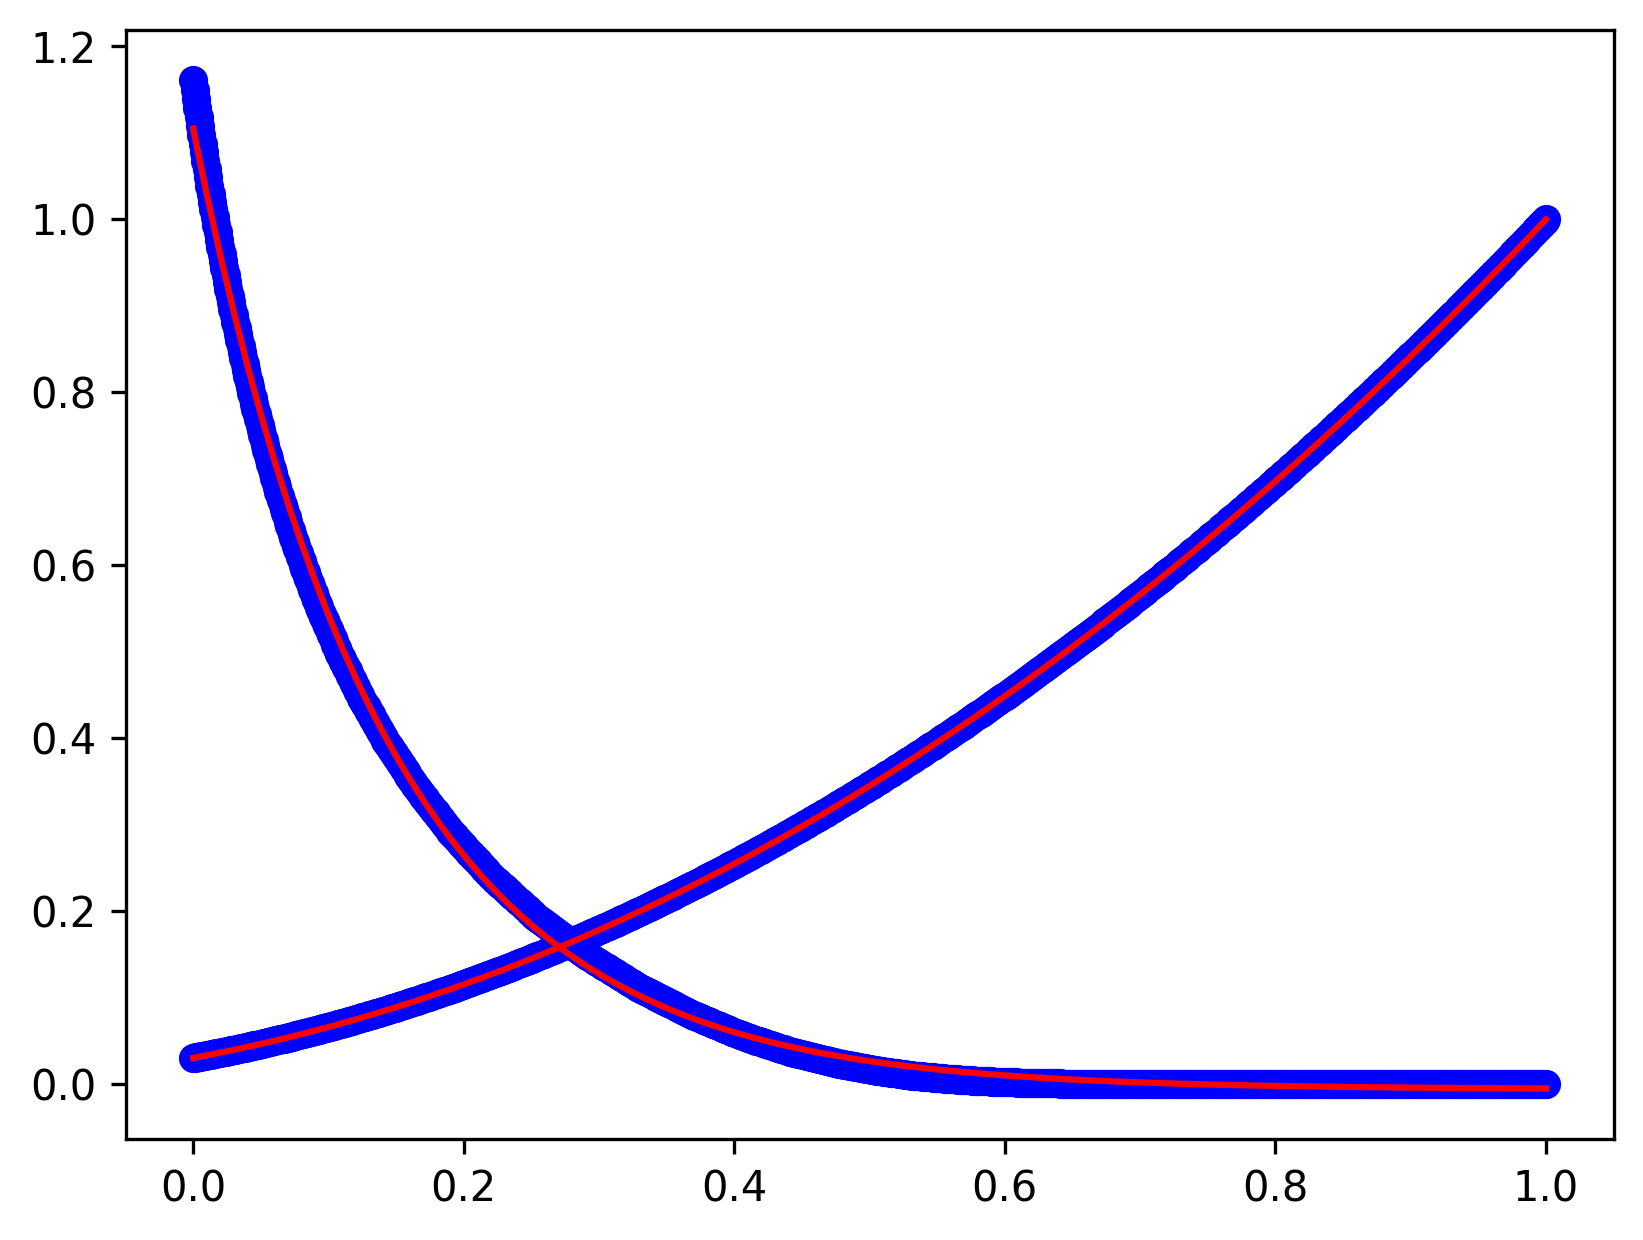
\includegraphics[width=0.8\linewidth]{images/fitted.png}
    \caption{Fitted $A(s)$ and $B(s)$ equations (red) with discrete values (blue) against the normalized annealing fraction $s$.}
    \label{fittedequation}
\end{figure}